\section{Overcoming the Limitations}
\subsection{Obviate GB computation}
Elimination ideal with ATO technique requires a GB computation, which is usually infeasible on large designs.
To obviate GB computation, we introduce a refinement on ATO as well as bit-word substitution method.

To overcome high computational complexity of GB calculation, \cite{pruss:dac14} proposed a
\underline{r}efinement of ATO (called RATO), and simplified the
\Grobner basis computation. They exploited Buchberger's product
criteria \cite{productc:1979}, which states that: {\it If the leading  
monomials of $f_i, f_j$ are relatively prime, then $Spoly(f_i, f_j)$
reduces to zero modulo the generating set, i.e. $Spoly(f_i, f_j)
\xrightarrow{F} _+ 0$.} This concept was exploited in RATO as follows: 

Perform a reverse topological sorting of the nodes in the
combinational logic, and define a {\it lex} term order by the
following relation $>_{r}$: {\it bit-level circuit variables ordered
  reverse topologically} $>$  {\it word-level output variables} $>$
{\it word-level input   variables}. Representing the polynomial ideal
$J$ in RATO has the effect that there exists {\it one and only one
  pair of polynomials} in $J$ that do not have relatively prime
leading terms (see  Section 5 in \cite{pruss:dac14} for details). All
other polynomial pairs will have leading terms that are 
relatively prime, so these polynomial pairs are not considered in
Buchberger's algorithm.  The authors of \cite{pruss:dac14} exploited
this concept and showed how the \Grobner basis of $(J + J_0)$ can be
computed by a {\it subset} of polynomials, which  improves the
scalability of their approach. Their approach, however, cannot
circumvent the \Grobner basis computation altogether. Consequently, 
their approach fails to derive a canonical polynomial abstraction when
the representation is dense, and contains monomials of high-degrees
(e.g. in case of buggy designs). 

Additionally, further improvements can be made to RATO:
With only RATO, the final remainder $h$ contains both bit-level variables and
word-level {\it state variables}. We desire
a polynomial in only word 
level variables without computing a
\Grobner basis. This can be achieved if we  represent the
bit-level state variables in terms of their word-level
variables. The basic idea of this improvement is: exploit the property of
polynomial squaring in $\Fkk$ to list $k$ polynomial equations,
use a Gaussian-elimination style technique to solve the system of equations.
Then we can substitute all bit-level variables in the remainder polynomial from RATO.
Details are described in our accepted DATE 2015 conference paper 
``{\it Formal Verification of Sequential Galois Field Arithmetic Circuits using Algebraic Geometry}".

\subsection{Complexity of multivariate division}
Using RATO and bit-word substitution, we can turn GB computation problem to a single multivariate division.
Although we gain success on verifying sequential GF multipliers, there are still problems when
doing implicit state enumerating on generic FSM. For example, when we tried to apply our approach
on ISCAS'89 benchmark s953 with 29 DFFs and 311 gates, RATO spent too much time on reducing
Spoly with ideal generators. By analyzing the process of polynomial reduction, we conjecture that
\begin{Conjecture}
Long chains of AND/OR gates will make polynomial reduction infeasible.
\end{Conjecture}

\begin{figure}[hbt]
\centering{
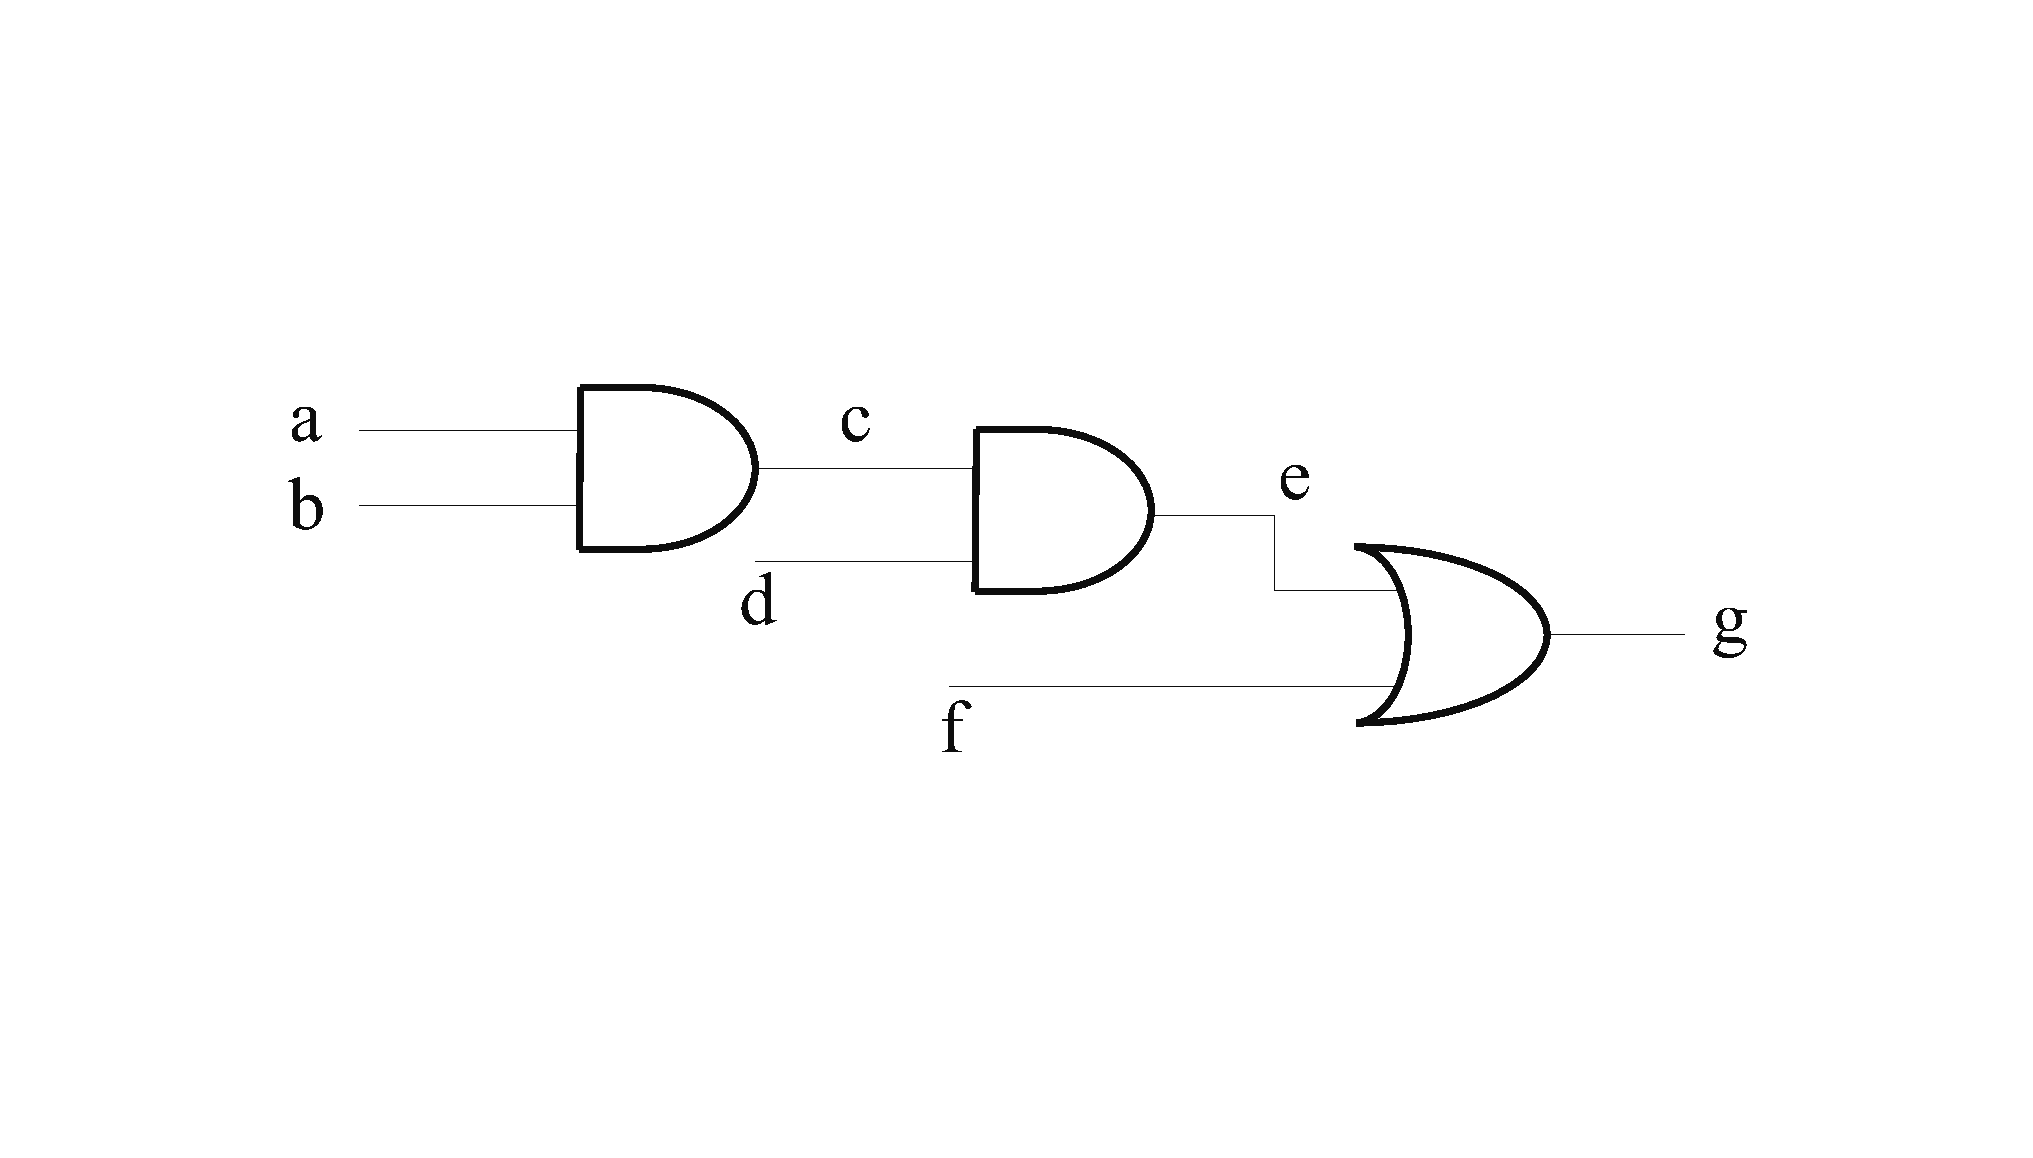
\includegraphics[scale=0.3]{./fig_chain.eps}
\caption{An example of AND-OR-gate chain}
\label{fig:chain}}
\end{figure}

\begin{Example}
Consider a chain (Fig.\ref{fig:chain}) of 3 gates: 2 AND gates and 1 OR gate. Write them in polynomials:
\begin{align*}
&h_1:g+ef+e+f\\
&h_2:e+cd\\
&h_3:c+ab
\end{align*}
Impose RATO: $g>e>c>\{a,b,d,f\}$. Reduce a simple polynomial $g$ with this set of polynomials:
$$g\xrightarrow{h_1}_{+} ef+e+f$$
$$g\xrightarrow{h_2}_{+} cdf+cd+f$$
$$g\xrightarrow{h_3}_{+} abdf+abd+f$$
We can conclude that:
\begin{itemize}
\item[-] When divided by polynomial from XOR gate, the length of remainder will increase by 1 term;
\item[-] When divided by polynomial from AND gate, the degree of remainder will increase by 1;
\item[-] When divided by polynomial from OR gate, the length and degree of remainder will increase by 1.
\end{itemize}
Since all gate polynomials have leading term with degree 1, a higher degree of remainder polynomial means
 more iterations of division (while a longer remainder does not always imply more divisions because
 there is still possibility to cancel multiple terms at one time). 
 Consider the querying time, a chain with AND/OR gates will blow up computational complexity of
reduction.

Sequential GF multiplier has only limited levels of gate chains (4 for RH-multiplier example). Although the size of 
datapath is large, actual complexity for reduction is relatively low.
\end{Example}

To lower down the complexity of reduction, we can introduce a matrix-based technique named as "F-4 style reduction" \cite{F4reduce}. 
It can speed up the procedure dividing a low-degree polynomial with term-sparse polynomial ideal. 

Another option is to cut back the cost of each univariate division. Horner's expansion diagram (HED)\cite{alizadeh2010modular}
is a graphical method to turn operations such as uniting like terms to lower complexity DAG manipulations.

